\chapter{Grundlagen}
\label{cha:Grundlagen}
Im folgenden werden für diese Arbeit notwendige Grundlagen zu unterschiedlichen Technologien und Wissensbereiche erarbeitet. 
Zuerst wird die menschliche Wahrnehmung erläutert, da auf diesen die Kriterien zur Evaluierung der Komponenten klassifiziert werden. Anschließend werden die Technologien der Komponenten des Prototypen vorgestellt, um einen Einblick auf die Funktionsweise zu liefern. Mit den technischen Grundlagen können Kriterien zur Bewertung der Technologien aufgestellt werden. Zuletzt werden die vorhandenen Bussysteme in Fahrzeugen vorgestellt und miteinander verglichen.
\section{Menschliche Wahrnehmung}
Menschliche Wahrnehmung ist die \glqq Tätigkeit oder Vorgang der Informationsaufnahme durch unsere Sinne\grqq{} \cite[Seite 12]{Buhler.2017}. Dieser Prozess beschränkt sich dabei nicht nur auf die Aufnahme von Informationen, sondern auch auf die Auswahl und Bewertung der Informationsdaten nach Relevanz. Die Aufnahme der Informationen geschieht über Sinnesorgane, die die Informationen über unterschiedliche Techniken in Reize wandeln. Die Auswahl und Bewertung erfolgt hauptsächlich im zentralen Nervensystem und dem Gehirn. \cite[Vgl. Seite 12]{Buhler.2017}\\
Mit 70 \% der wahrgenommenen Umweltreize ist das Auge, das bedeutendste Sinnesorgan des Menschen vor der Haut, Nase, Ohr oder Zunge. Unsere Wahrnehmung ist dabei immer eine Interpretation der erhaltenen Sinnesreize aller Sinnesorgane. Unsere visuelle Wahrnehmung ist daher nicht nur durch die Augen bestimmt, sondern auch durch die Ohren, der Nase, der Zunge und der Haut. Daneben spielen unsere Erfahrungen und emotionale Lage einen Einfluss auf die Wahrnehmung. \cite[Vgl. Seite 13 f.]{Buhler.2017}
Abbildung \ref{fig:information} veranschaulicht diesen Zusammenhang mit optischen Informationsaufnahme über die Physik, Physiologie und der Psychologie. \\
\begin{figure}[hbt]
	\centering
	\begin{tikzpicture}[first style/.style={rectangle, rounded corners, align=center}, steuer style/.style={draw, rectangle, text width=2.8cm, align=center}]
	\shade[left color=cyan!30!white, right color=blue!40!white] (1, 5.5) rectangle (8,-3);
	\shade[left color=green!30!white, right color=cyan!30!white] (-5, 5.5) rectangle (1,-3);
	\draw (-3, 3) arc (-170:170:12mm);
	\draw[very thick] (-2.4, 2.25) arc (-120:120:11mm) ;
	\draw[->, red] (-5, 3.2) -- node[above] {Licht} (-3.5 , 3.2);
	\node[first style] (A) at (-2, 4.6) {Auge};
	\node[first style, ultra thick] (P1) at (-4, 5){\textbf{Physik}};
	\node[first style, ultra thick] (P2) at (1, 5){\textbf{Physiologie}};
	\node[first style, right=of P2, ultra thick] (P3) at (4, 5) {\textbf{Psychologie}};
	\node[steuer style] (S6) at (5, 3.5) {Nervöse Filtersteuerung};
	\node[steuer style, thick] (S1) at (5, 0) {Wahrnehmung};
	\node[steuer style] (S5) at (1, 1.5) {Nervöse Informationsverarbeitung};
	\node[steuer style] (S2) at (5, -2)  {Stimmungen und Gefühle};
	\node[steuer style] (S4) at (1, 0) {Andere Sinnesorgane};
	\node[steuer style] (S3)  at (1, -2) {Gespeicherte Erfahrung};
	\draw[very thick] (S5) -- (-0.8, 2.9);
	\draw (S1) -- (S2);
	\draw (S1) -- (S3);
	\draw (S1) -- (S4);
	\draw (S1) -- (S5);
	\draw (S1) -- (S6);
	\draw (S5) -- (S6);
	\draw (S2) -- (S3);
	\draw (S4) -- (S3);
\end{tikzpicture}
	\caption[Visuelle Wahrnehmung]{Visuelle Wahrnehmung}
	\label{fig:information}
\end{figure}
Ein bekanntes Beispiel für das Zusammenwirken zwischen den Sinnen, ist die Ausrichtung der Augen und des Kopfes durch das Hören von besonderen Geräuschen, wie einer Explosion.\\
Das bedeutet, dass die Wahrnehmung ganzheitlich betrachtet werden muss, da die einzelnen Wahrnehmungsarten miteinander in Wechselwirkung stehen. \\
Mit Medien können visuelle, auditive, haptische, motorische und olfaktorische Sinneskanäle angesprochen werden. Das Ziel der Medien ist dabei die Aufmerksamkeit des Menschen auf das Objekt zu richten und den erwünschten Einfluss auf den Menschen zu schaffen. Visuelle Inhalte können Schriften, Grafiken, Animationen oder Farben sein. Auditive sind Musik oder Geräusche. Haptische Inhalte sind fühlbare Strukturen und Oberflächen, während motorische Inhalte bewegliche Teile sind. Olfaktorische Reize sind Düfte und Gerüche. \cite[Vgl. Seite 3]{Buhler.2017}\\
In den nächsten Unterkapiteln werden die unterschiedlichen menschlichen Wahrnehmungsarten vertieft erläutert. Der Fokus ist auf die visuelle Wahrnehmung gerichtet, da dort der Schwerpunkt der späteren Arbeit liegt. Zu allen Wahrnehmungen wird auf die Physiologie der Sinne eingegangen und für diese Arbeit relevante Details.
\subsection{Visuelle Wahrnehmung}
Die visuelle Wahrnehmung basiert hauptsächlich auf den Sinneseindrücken durch unser Auge und daneben, wie oben erwähnt, aus dem Zusammenspiel der anderen Sinnesorgane. \\
Das Auge besitzt lichtempfindliche Zellen. Die Zellen werden dabei zwischen Stäbchen und Zapfen unterschieden. Die Mehrzahl an Zellen bilden die spektral unempfindlichen Stäbchen, mit ca. 120 Millionen pro Auge, während nur eine geringe Anzahl von 7 Millionen pro Auge farbempfindliche Zapfen sind. Durch den Unterschied in der Anzahl ist das Sehen bei Dunkelheit eher schwarz-weiß, da die Anzahl der Zapfen nicht ausreicht, um genügend Licht zu erhalten und ein Farbbild zu erzeugen. Dabei ist ein Zapfen immer nur für eine der drei licht Frequenzbereiche rot (langwellig), grün (mittelwellig) oder blau (kurzwellig) lichtempfindlich. Die Farben in der menschlichen Wahrnehmung sind daher ein Ergebnis der Signalverarbeitung der drei unterschiedlichen Zapfenarten. \cite[Vgl. Seite 14]{Buhler.2017}\\
Abbildung \ref{fig:Auge} zeigt eine schematische Darstellung eines Auges mit der Vergrößerung eines Teilbereiches. In dem Teilbereich sind die Stäbchen und Zapfen dargestellt. \\
\begin{figure}[hbt]
	\centering
	\includegraphics[width=0.5\linewidth]{images/Auge}
	\caption[Schematische Darstellung eines Auges mit den Nervenzellen]{Schematische Darstellung eines Auges mit den Nervenzellen \cite[Seite 141]{Schonhammer.2013}}
	\label{fig:Auge}
\end{figure}
Menschen können dabei nicht von ihrem Standpunkt aus den gesamten Raum betrachten, sondern durch biologischen Gegebenheiten immer nur ein Feld. Das Blickfeld deckt in der Horizontalen ca. 180\,° und in der Vertikalen 120\,° ab. Von diesem Blickfeld sind nur ca. 1,5\,° in beiden Dimensionen als scharfes Bild sichtbar. \\
Durch Bewegungen des Auges und des Kopfes werden verschiedene scharfe Bereiche abgedeckt. Unser Gehirn fügt diese Bereiche zusammen, um ein ganzheitliches scharfes Blickbild zu erzeugen. \cite[Vgl. Seite 14]{Buhler.2017}
Interessant für die Bewertung der optischen Komponenten ist das Sehvermögen des Auges, Pixel bei einer bestimmten Distanz noch zu erkennen. Das Auflösungsvermögen beschreibt den kleinsten Winkel zwischen zwei Punkten, die noch als getrennt wahrgenommen werden. In der Literatur wird das Auflösungsvermögen A\nomenclature{A}{Auflösungsvermögen} des menschlichen Auges auf $ 1' = \frac{1}{3000}\,\mathrm{°} = 0,0167\,\mathrm{°} $ angegeben. Mithilfe von trigonometrischen Rechnungen kann der Abstand x der zwei Punkte bei einer bestimmten Entfernung d und die dazu gehörige Pixeldichte ppi berechnet werden. die Bezugslänge $ d_{i} $ für die Pixeldichte ist häufig ein Inch. \cite[Vgl. Seite 209 f.]{LofflerMang.2020}
\begin{align}
	x &= \sin (A) \cdot d \\
	ppi &= \frac{d_{i}}{x}
\end{align}
Die Tabelle \ref{tab:Aufloessung} zeigt eine Aufstellung über die Entfernung zwischen dem Auge und der Oberfläche mit der benötigten Pixeldichte.
\begin{table}[hbt]	
	\centering
	\renewcommand{\arraystretch}{1.5}	% Skaliert die Zeilenhöhe der Tabelle
	\captionabove[Berechnung der benötigten Pixeldichte bei einer bestimmten Entfernung]{Berechnung der benötigten Pixeldichte bei einer bestimmten Entfernung}
	\label{tab:Aufloessung}
	\begin{tabular}{c|c}
		\parbox[t]{0.2\linewidth}{\centering Entfernung} & \parbox[t]{0.2\linewidth}{\centering Pixeldichte}  \\
		\hline 
		\hline 
		$ 0,3\,\mathrm{m} $ & $ 291\,\mathrm{ppi} $ \\
		$ 0,5\,\mathrm{m} $ & $ 175\,\mathrm{ppi} $ \\
		$ 1,0\,\mathrm{m} $ & $ 87\,\mathrm{ppi} $ \\
		$ 2,0\,\mathrm{m} $ & $ 44\,\mathrm{ppi} $ \\
		$ 3,0\,\mathrm{m} $ & $ 29\,\mathrm{ppi} $ \\
		$ 5,0\,\mathrm{m} $ & $ 17\,\mathrm{ppi} $ \\
		$ 8,0\,\mathrm{m} $ & $ 11\,\mathrm{ppi} $ \\
		$ 10\,\mathrm{m} $ & $ 9\,\mathrm{ppi} $ \\
	\end{tabular} 
\end{table}
%\cite[Vgl. Seite 142 ff.]{Schonhammer.2013}%
\subsection{Haptische Wahrnehmung}
Die haptische Wahrnehmung ist ein Teilbereich der Somatosensorik. Die Sinneszellen der Somatosensorik werden in drei Bereiche eingeteilt:
\begin{itemize}
	\item Exterozeption, Wahrnehmung der Außenwelt
	\item Propriozeption, Wahrnehmung der Stellung der Gliedmaßen
	\item Interozeption, Wahrnehmung des inneren Körpers
\end{itemize}
Die somatosensorische Wahrnehmung verbindet diese drei Arten, die zum Teil bewusst oder unbewusst vom Körper aufgenommen werden. Besonders relevant für diese Arbeit im Bereich der haptischen Wahrnehmung ist die Exterozeption beziehungsweise die Oberflächensensibilität. \cite[Vgl. Seite 26]{Sprenger.2020}\\
Die haptische Wahrnehmung erfolgt durch Rezeptoren in der Haut, die die Form, Oberfläche und Position von Objekten registrieren. Die Rezeptoren können unterschieden werden in
\begin{itemize}
	\item Thermorezeptoren für relative Temperaturunterschiede zur Körperbefindlichkeit, 
	\item Chemorezeptoren für Stoffe,
	\item Nozirezeptoren für starke Temperaturunterschiede oder Drücke bis zur Gewebeschädigung und
	\item Mechanorezeptoren für Empfindung von Oberflächen und Druck.
\end{itemize}
Die Mechanorezeptoren können wiederum in unterschiedliche Arten eingeteilt werden, die auf Druck, Berührung oder Vibration reagieren. \cite[Vgl. Seite 26 f.]{Sprenger.2020} \\
Eine Übersicht bietet die Grafik \ref{fig:hapWahrnehmung}. Oben sind die unterschiedlichen Rezeptoren für die haptische Wahrnehmung zu sehen, während unten die Einteilung der Sinneszellen in die unterschiedlichen Wahrnehmungsarten erfolgt.
\begin{figure}[hbt]
	\centering
	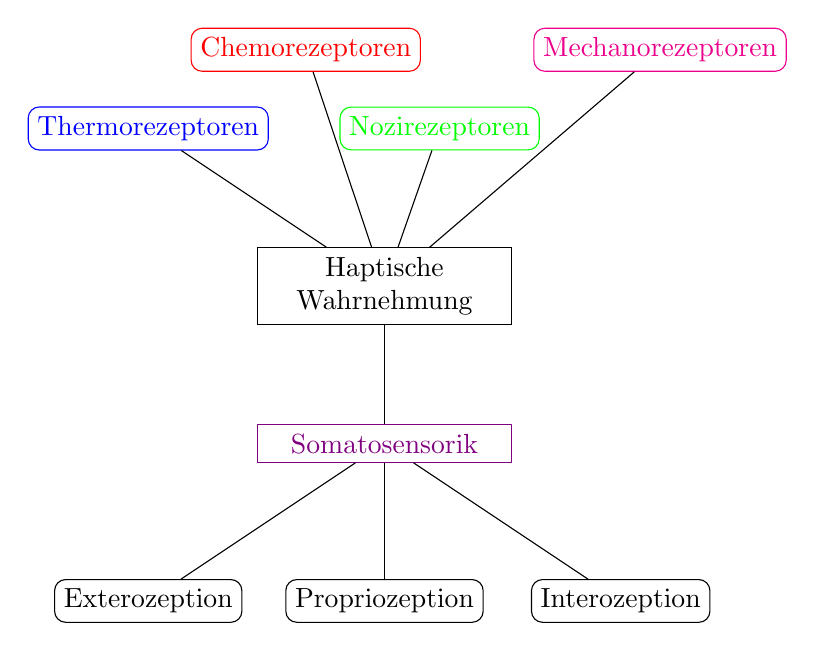
\begin{tikzpicture}[first style/.style={rectangle, draw, rounded corners, align=center}, steuer style/.style={draw, rectangle, text width=3cm, align=center}]
	\node[steuer style] (S1) at (0, 0) {Haptische Wahrnehmung};
	\node[steuer style, violet] (S2) at (0, -2) {Somatosensorik};
	\node[first style] (S3) at (-3, -4) {Exterozeption};
	\node[first style] (S4) at (0, -4) {Propriozeption};
	\node[first style] (S5) at (3, -4) {Interozeption};
	\node[first style, blue] (S6) at (-3, 2) {Thermorezeptoren};
	\node[first style, red] (S7) at (-1, 3) {Chemorezeptoren};
	\node[first style, green] (S8) at (0.7, 2) {Nozirezeptoren};
	\node[first style, magenta] (S9) at (3.5, 3) {Mechanorezeptoren};
	\draw (S1) -- (S2);
	\foreach \y in {3,...,5}
	\draw (S2) -- (S\y);
	\foreach \x in {6,...,9}
	\draw (S1) -- (S\x);
\end{tikzpicture}
	\caption[Haptische Wahrnehmung]{Haptische Wahrnehmung}
	\label{fig:hapWahrnehmung}
\end{figure}
Die Verteilung der unterschiedlichen Rezeptoren ist im Körper ungleichmäßig. In der Handinnenflächen gibt es zum Beispiel Areale mit unterschiedlicher Empfindsamkeit \glqq auf Druckintensität, Geschwindigkeit einer Veränderung an der Haut oder einer Vibration. \grqq{} \cite[Seite 29]{Sprenger.2020}\\
Die Empfindungsschwelle gibt Auskunft darüber, wie stark eine Hautstelle gedrückt werden muss, damit eine Berührung wahrgenommen wird. Durch das Berühren der Haut mit zwei Tastpunkten in bestimmter Entfernung kann das räumliche Auflösungsvermögen bestimmt werden. \cite[Vgl. Seite 28]{Sprenger.2020}\\
Die Wahrnehmung von Oberflächen geschieht über alle Sinneseindrücke. Zuerst werden die Hauptmerkmale Oberflächenstruktur, wie glatt oder rau, wahrgenommen und die Größe des Objektes durch die visuelle Wahrnehmung erfasst und im zweiten Schritt die gefühlte Temperatur. \cite[Vgl. Seite 33]{Sprenger.2020}\\
\glqq Die Verknüpfung der haptischen Wahrnehmung mit projizierten Simulationen zeigt letztendlich den Wunsch nach Kombinationen zu multisensuellen Interfaces, die allerdings nicht mehr die audiovisuelle Wahrnehmung als strikt dominant betrachten und die haptische Wahrnehmung ausschließlich als unterstützenden Sinn zur verbesserten Immersion heranziehen. Über die Haptik sollen direkt und unabhängig von anderen Sinnen Informationen gegeben wie auch erfahren werden, die in Kombination mit den anderen Sinnen kräftigere Informationsträger sind und somit auch als multisensuelle Kombinationen erforscht werden. \grqq{} \cite[Seite 263]{Sprenger.2020}
\subsection{Akustische Wahrnehmung}
Der Mensch ist in der Lage mit den Ohren Schallwellen zwischen 20 Hertz und 20 Kilohertz zu hören. Schallwellen sind Druckwellen eines Mediums wie Luft oder Wasser in longitudinaler Richtung. Das bedeutet, die Druckamplitudenrichtung ist parallel zur Ausbreitungsrichtung. \cite[Vgl. Seite 217]{Schonhammer.2013} \\
\glqq Über den äußeren Gehörgang gelangt die Schallwelle zum Trommelfell. Die Schwingungen des Trommelfells werden über die Kette der drei Gehörknöchelchen (Hammer, Amboss, Steigbügel) an das ovale Fenster übertragen, dessen Membran die mit Flüssigkeit gefüllte Schnecke (Cochlea) abschließt. Die Cochlea ist ein schneckenförmiger Kanal, der in das überaus harte Felsenbein eingebettet ist und die Basilarmembran enthält. Schallschwingungen erregen eine längs dieser Membran entlang fortschreitende Welle. Durch diese Auslenkung der Basilarmembran werden die Haarzellen angesprochen, die in einem geometrischen Muster längs der Basilarmembran angeordnet sind und das Muster der Anregung an das Gehirn übertragen. \grqq{} \cite[Seite 71f.]{Bernstein.2019}
Das Bild \ref{fig:Ohr} zeigt einen schematischen Aufbau des Gehörgangs mit den oben beschriebenen Teilen.
\begin{figure}[hbt]
	\centering
	\includegraphics[width=0.7\linewidth]{images/Ohr}
	\caption[Schematische Darstellung des Gehörgangs mit den unterschiedlichen Bereichen]{Schematische Darstellung des Gehörgangs mit den unterschiedlichen Bereichen \cite[Seite 219]{Schonhammer.2013}}
	\label{fig:Ohr}
\end{figure}
\subsection{Olfaktorische Wahrnehmung}
Unser Körper ist in der Lage Gerüche schon bei sehr geringen Konzentrationen zu unterscheiden und Unterschiedlichkeiten wahrzunehmen. In der menschlichen Nase befinden sich Riechzellen in der Riechschleimhaut. Durch chemische Reize in den Rezeptoren der Zellen werden spezifische Entladungsmuster an evolutionär ältere Gehirnareale und das limbische System gesendet. Das limbische System ist maßgeblich für die Emotionen des Menschen verantwortlich. \cite[Vgl. Seite 102]{Schonhammer.2013}\\
Gerüche werden oft nach dem Stoff benannt mit dem sie assoziiert werden, zum Beispiel ein blumiger Geruch bei Gerüchen, die dem Geruch von Blumen ähneln. Diese Klassifikation bei Gerüchen ist dabei nicht eindeutig, da die Zuordnung von Gerüchen mit Objekten Überschneidungen mit anderen Gerüchen haben können. Eine bessere Differenzierung von Gerüchen in Kategorien ist die Bewertung von Gerüchen nach angenehm und unangenehm. Da die olfaktorische Wahrnehmung und Gefühle eng miteinander verbunden sind. Angenehme Gerüche verursachen eine positive Stimmung und eine anziehende Gestik. \cite[Vgl. Seite 105 f.]{Schonhammer.2013}\\
Paul Jellinek klassifiziert Gerüche auf einer zweidimensionalen Karte \ref{fig:Duft} zischen süß - bitter und basisch - sauer. \cite[Vgl. Seite 104]{Schonhammer.2013}
\begin{figure}[hbt]
	\centering
	\includegraphics[width=0.5\linewidth]{images/Duft}
	\caption[Duftkreis nach P. Jellinek]{Duftkreis nach P. Jellinek \cite[Seite 105]{Schonhammer.2013}}
	\label{fig:Duft}
\end{figure}
\glqq Konzepte zur Beduftung der Innenräume von Automobilen werden u.a. unter dem Aspekt des allgemeinen Erregungszustandes des Fahrers vertreten. Gemeinsam mit Beleuchtung und Beschallung sollen Düfte den Menschen am Steuer etwa stimulieren oder beruhigen.\grqq{} \cite[Seite 122 f.]{Schonhammer.2013}\\
\glqq Beduftung mag als verlockende Strategie emotional wirksamer Gestaltung erscheinen, ist jedoch nicht nur aus ethischen Gründen, sondern in Rücksicht auf das Wohlbefinden unfreiwillig Betroffener problematisch. [...] Schließlich ist daran zu erinnern, dass wegen der innigen Verbindung von Gefühl und Geruch Momente der visuellen, akustischen und taktil-haptischen Gestaltung indirekt auch auf das Riechen wirken. \grqq{} \cite[Seite 123]{Schonhammer.2013}
\section{Technologien}
In den folgenden Unterbereichen werden jeweils die einzelnen Technologien, die in dieser Arbeit behandelt werden, auf Funktionsweise, Beschaffenheit und Aufbau vorgestellt. Daneben werden die wichtigsten Kenngrößen zur Beurteilung der Technologien erläutert.
\subsection{Lumineszenzdiode}
Lumineszenzdioden (LED\nomenclature{LED}{Lumineszenzdiode}) sind lichtemittierende Dioden, die Strahlen im sichtbaren oder infraroten Spektralbereich erzeugen. Dioden sind die einfachste Form von elektronischen Bauteilen und bestehen aus dotierten Halbleitermaterial mit einer pn-Schicht. Das Halbleiter-Grundmaterial bestimmt den abgestrahlten Spektralbereich des Lichtes. Liegt eine Spannung in Durchlassrichtung der Dioden an, strahlt diese in ihrem Frequenzbereich Photonen ab. \cite[Vgl. Seite 193 f.]{LofflerMang.2020} \\

%*Ein einfaches Beispiel soll den Zusammenhang zwischen Material und Farbe des emittierten Lichts verdeutlichen. Für die Energie von Photonen gilt nach der Einstein\grq schen Gleichung:
%\begin{equation}
%	E = h \cdot f = \frac{h \cdot c}{\lambda}
%\end{equation}
%Die Energie eines Photons ist das Produkt des Plank\grq schen Wirkungsquantums $ h = 6,626 \cdot 10^{-34}\, \mathrm{Js} $ und der Lichtgeschwindigkeit $ c = 299792458\, \frac{\mathrm{m}}{\mathrm{s}}$ durch die Wellenlänge $ \lambda $ des Photons.
%Durch Umstellung folgt die Wellenlänge des Photons:
%\begin{equation}
%	\lambda = \frac{c \cdot h}{E}
%\end{equation}
%Galliumphosphid hat zum Beispiel eine Bandlücke von $ 2,25\,\mathrm{eV} $, wodurch Licht mit der Wellenlänge von
%\begin{equation}
%	\lambda = \frac{c \cdot h}{E} = \frac{6,626 \cdot 10^{-34}\,\mathrm{Js} \cdot 299792458\,\frac{\mathrm{m}}{\mathrm{s}}}{2,25 \cdot 1,602 \cdot 10^{-19}\, \mathrm{J}} = 551\,\mathrm{nm}
%\end{equation}
%im blau-grünen Spektrum emittiert wird. 
Die meisten LEDs sind SMD-Bauteile (Surface-mounted device\nomenclature{SMD}{Surface-mounted device}) und sitzen in einem Kunststoff-, Keramik- oder Epoxidharzgehäuse. 
Um eine Hintergrundbeleuchtung mit Hilfe von LEDs zu erzeugen kann ein Leuchtkörper mit einer Vielzahl an LEDs hinter einer Streulichtscheibe verbaut werden, wodurch ein gleichmäßiges Licht entsteht. \cite[Vgl. Seite 194]{LofflerMang.2020} \\
Zum Erzeugen von weißem Licht strahlen drei verschiedene LEDs mit den Farben rot, grün und blau gleich hell und erst im Auge entsteht durch die Kombination ein weißes Licht. Da hier aber drei LEDs genutzt werden, ist diese Variante teurer. Der Vorteil ist, dass bei variabler Einstellung der Helligkeit der einzelnen Dioden unterschiedliche Farben für den Betrachter angezeigt werden können. \\ 
Günstiger sind Weißlicht-LEDs (WLED\nomenclature{WLED}{Weißlicht-LED}), bei denen in der Produktion auf Basis von blauen LEDs noch ein fluoreszierender Konverterstoff beigemischt wird. Dieser Stoff wird durch das blaue Licht angeregt und strahlt einen breiten Spektralbereich wieder aus, wodurch ein weißes Licht aus Primär- und Sekundärlicht entsteht. Bei WLEDs ist die Farbe nicht variabel. \cite[Vgl. Seite 194]{LofflerMang.2020} \\
Organische LED (OLED\nomenclature{OLED}{Organische LED}) besitzen einen veränderten Schichtaufbau, bei dem zwischen p- und n-Schicht eine organische Schicht aufgebracht ist. OLEDs sind dünner als normale LEDs und dadurch leichter und flexibel, wodurch sich neue Einsatzbereiche ergeben. Daneben besitzen sie eine hohe Helligkeit bei starkem Kontrast. \cite[Vgl. Seite 195]{LofflerMang.2020}
\subsection{LED-Matrix}
Eine LED-Matrix ist eine bestimmte Anordnung von LEDs in zwei orthogonalen Richtungen auf einer Ebene. Somit entsteht ein zwei dimensionales Bild.\\ 
Die Pixeldichte beschreibt, wie viele einzelne LEDs auf einer bestimmten Fläche sind. Häufig wird die Größe \glqq pixels per inch\grqq{} (ppi\nomenclature{ppi}{parts per inch}) herangezogen. Je näher der Betrachter an der Anzeigefläche steht, desto höher muss die Pixeldichte sein, damit der Betrachter einzelne Pixel nicht erkennt.
\subsection{Bildschirmtechnologien}
Unter den Bildschirmtechnologien werden folgend zwei unterschiedliche Realisierungen vorgestellt. Die erste Technologie sind aktive OLED-Displays und die Zweite passive Flüssigkristallanzeigen (LCD\nomenclature{LCD}{Flüssigkristallanzeigen}). \\
Durch die schnellen Entwicklungen bei Bildschirmtechnologien ist es nicht möglich, alle unterschiedlichen Techniken vorzustellen. Die folgenden Absätze sollen ein Grundverständnis für die möglichen Funktionsweisen liefern.\\
Aktiv bedeutet in diesem Fall, dass die Pixel das Licht selbst erzeugen, während passive Displays auf ein Hintergrundlicht angewiesen sind, da sie nur Licht abdunkeln oder durchlassen können. \\
\glqq OLED-Displays bestehen aus einem zweidimensionalen Array weißes Licht abstrahlender OLEDs, denen Farbfilter (RGB) vorgelagert sind.\grqq \cite[Seite 347]{LofflerMang.2020} Eine weitere Möglichkeit wären OLEDs mit unterschiedlichen Grundfarben (rot, grün und blau), die zusammen ein Pixel erzeugen. \\
Flüssigkristallanzeigen besitzen einen mehrschichtigen Aufbau. Die Zentrale Schicht ist eine Flüssigkristallschicht, die bei Anlegen einer Spannung an den Elektrodenschichten der Flüssigkristalle ausrichtet und die Polarisierung des einfallenden Lichtes in eine bestimmte Richtung lenkt, sodass das Licht bei einem nach geführten Polarisationsfilter entweder absorbiert oder transmittiert wird. \cite[][Vgl. Seite 346 f.]{LofflerMang.2020} Je nach Ausführung kann das Licht bei angelegter Spannung oder spannungslos transmittieren. Die Richtung und Technik der Beleuchtung der LCD variiert je nach Technik.
\subsection{Videoprojektoren}
Videoprojektoren können auf Basis unterschiedlicher Technologien für die Situation angepasst eingesetzt werden. Unterschiedliche Arten von Projektoren sind zum Beispiel LCD-, DLP- (Digital Light Processing\nomenclature{DLP}{Digital Light Processing}), LED-, LCoS- und Laser-Projektoren. \\
Zu Unterscheidung von Projektionsverfahren können diese wieder in aktive und passive Systeme eingeteilt werden. Heutzutage werden vorwiegend passive Systeme, sogenannte Lichtventilprojektoren, eingesetzt. \cite[Vgl. Seite 551]{Schmidt.2021} \\
Für die Auswahl des richtigen Projektors ist die Einsatzumgebung von Bedeutung. Je nach Helligkeit des Raumes ist die Helligkeit und der Kontrast unterschiedlich auszuwählen. Bei hoher Umgebungshelligkeit ist ein Projektor mit hoher Helligkeit vorzuziehen. Dabei ist ein niedrigerer Kontrast durch die Aufhellung der dunklen Bildbereiche durch das Umgebungslicht nicht negativ. \cite[Vgl. Seite 562]{Schmidt.2021}
\subsection{Elektronisches Papier}
Elektronisches Papier (E-Papier\nomenclature{E-Papier}{Elektronisches Papier}) ist eine Bezeichnung für Bildschirme, deren visuelle Anmutung Papier entspricht und deren Inhalt durch Elektronik gesteuert wird. Häufig sind diese Displays passiv, also reflektieren nur Licht und erzeugen keines. Bei manchen E-Papieren ist seitlich eine Hintergrundbeleuchtung, die über eine Folie das Display beleuchtet. Im folgenden wird die häufig verwendete Technologie der Elektrophorese für die Displays erläutert. \\
\glqq Elektronisches Papier lässt sich vereinfacht als dünne, flexible Folie beschreiben, in der in Flüssigkeit eingelagerte, elektrisch geladene Partikel (als elektronische Tinte bezeichnet) ein schwarz-weißes oder allgemein zweifarbiges Bild ergeben. Dies wird ermöglicht, indem über Elektroden elektrische Felder auf die Partikel wirken, die sich entsprechend der Ladung des angelegten Feldes ausrichten. \grqq \cite[Seite 568]{Schryen.2002} \\
%TODO Bild der schichten einbauen%
Pro Pixel eines Bildes wird eine Mikrokapsel genutzt in der sich mehrere positiv geladene weiße Partikel und negativ geladene schwarze Partikel befinden. Auf beiden Seiten der Folie befinden sich Elektroden, wovon eine auf der Betrachtungsseite transparent ist. Wird auf der transparenten Elektrode eine negative Spannung und auf der inneren Elektrode eine positive, richten sich die Mikrokapseln dementsprechend aus, dass die positiven Partikel nach außen zeigen. Das Bild ist dementsprechend weiß. \cite[Vgl. Seite 567 f.]{Schryen.2002} \\
E-Papiere benötigen nur beim Ändern der Polarität der Pixel elektrische Energie, wodurch der Strombedarf bei seltene Bildschirmänderungen gering ist. \\
Vorteile gegenüber LCD-Displays sind die niedrigeren Herstellungskosten, geringeres Gewicht und die bessere Lesbarkeit. \cite[Vgl. Seite 569]{Schryen.2002}
Da bei E-Papieren vorwiegend Bilder dargestellt werden, soll im folgenden die Berechnung der Dateigröße eines Bildes für ein mögliches E-Papier erläutert werden.
Als Beispiel dient ein Schwarz-Weiß E-Papier mit einer Farbtiefe von 16 Stufen. Die Farbtiefe $ FT $\nomenclature{FT}{Farbtiefe} beträgt bei 16 Stufen zwar nur 5 Bit, um aber auf gängige Datengrößen zu kommen, sollte für die Berechnung 8 Bit pro Pixel und damit 1 Byte angenommen werden. Das Dateiformat JPEG \nomenclature{JPEG}{Joint Photographic Experts Group} nutzt 8 Bit pro Farbkanal. Die Pixelanzahl pro Zeile $ P $ \nomenclature{P}{Pixelanzahl pro Zeile}beträgt 1920 Pixel und Zeilenanzahl $ Z $\nomenclature{Z}{Zeilenanzahl} 1080 Pixel. Der Komprimierungsfaktor $ KF $\nomenclature{KF}{Komprimierungsfaktor} ist eine Zahl, die angibt wie stark die reine Datenmenge des Bildes noch durch digitale Komprimierungsverfahren reduziert werden kann. Wir benutzen hier einen Komprimierungsfaktor von 12. \cite[Vgl. Seite 22]{Buhler.2018}
\begin{align}
		Datenmenge &= \frac{P \times PZ \times FT}{KF} \label{eq:Bilddatenmenge}\\
		&= \frac{1920\,\frac{\mathrm{Pixel}}{\mathrm{Zeile}}\times 1080\,\mathrm{Zeilen} \times 8\,\frac{\mathrm{Bit}}{\mathrm{Pixel}}}{12} \\
		&= 1382400\,\mathrm{Bit} = 1,3824\,\mathrm{MBit} = 172,8\,\mathrm{KByte}
\end{align}
\section{Bordnetz}
Moderne Fahrzeuge besitzen über 100 Steuergeräte verteilt im Fahrzeug. Zur Kommunikation zwischen den Steuergeräten werden unterschiedliche Bussysteme genutzt. \\
Im folgenden werden die gängigen Bussysteme in der Fahrzeugtechnik vorgestellt, um für den späteren Konzeptentwurf die notwendigen Grundlagen zu kennen. Im Anschluss erfolgt ein Vergleich zwischen den Merkmalen der einzelnen Bussysteme.
\subsection{Controller Area Network (CAN \nomenclature{CAN}{Controller Area Network})}
CAN wird zum Austausch von Mess-, Steuer- und Regelsignalen genutzt. Es ist ein bitstrom-orientiertes System. Es basiert auf Differenzsignalübertragung und benutzt dazu verdrillte Leiterpaare. Als ereignisgesteuertes System wird das Senden von Nachrichten durch ein Ereignis ausgelöst. \\
Der High-Speed CAN besitzt Bitraten von $ 250\,\frac{\mathrm{kBit}}{\mathrm{s}} $ bis zu $ 1\,\frac{\mathrm{MBit}}{\mathrm{s}}$.
Der Low-Speed CAN besitzt Bitraten kleiner als $ 125\,\frac{\mathrm{kBit}}{\mathrm{s}} $. 
Der CAN verfügt über Fehlererkennung und Sicherungssysteme. Das Senden von Nachrichten erfolgt über eine Priorisierung der Nachrichten. \cite[Vgl. Seite 57 ff.]{Zimmermann.2014}
\paragraph{Performance}
Je nach Ausschöpfung der Nutzdatenmenge pro Botschaft liegt die maximale Übertragungsgeschwindigkeit zwischen $ 7,7\,\frac{\mathrm{kByte}}{\mathrm{s}} $ bei einem Byte Nutzdaten pro Botschaft und $ 29,6\,\frac{\mathrm{kByte}}{\mathrm{s}} $ bei acht Byte Nutzdaten. Die Latenz einer Botschaft ist nicht deterministisch bestimmbar und ist abhängig von der aktuellen Buslast und der Priorität der Botschaft. Die Übertragungsdauer einer Botschaft mit maximaler Nutzdatenmenge bei $ 500\,\frac{\mathrm{kBit}}{\mathrm{s}} $ Bittakt liegt bei $ 270\,\mathrm{\mu s}$.
Durch den Einsatz der weiterentwickelten CAN-Version CAN FD (CAN with Flexible Data Rate\nomenclature{CAN FD}{CAN with Flexible Data Rate}) kann die Übertragungsgeschwindigkeit durch größere Nutzdatenmengen und höherer Bittakte auf bis zu $ 260\,\frac{\mathrm{kByte}}{\mathrm{s}} $ gesteigert werden. \cite[Vgl. Seite 76 ff.]{Zimmermann.2014}
\subsection{Local Interconnect Network (LIN\nomenclature{LIN}{Local Interconnect Network})} 
Der LIN soll mit einem einfacheren Aufbau eine kostengünstige Alternative zum CAN für Low Speed Sensor-Aktor Anwendungen bieten.
LIN ist ein Master-Slave gesteuertes Netzwerk, worin der Master die gesamte Kommunikation steuert, indem er die Slaves nach einem Zeitplan Berechtigungen zum Senden gibt. Die Bitrate beträgt üblicherweise $ 19,2\,\frac{\mathrm{kBit}}{\mathrm{s}} $
\cite[Vgl. Seite 79 ff.]{Zimmermann.2014}
\paragraph{Performance}
Für Botschaften mit acht Byte Nutzdaten werden Sendezeitraster von 10 ms benötigt. \cite[Vgl. Seite 94 f.]{Zimmermann.2014} Die Nutzdatenmenge beträgt dementsprechend ca. $ 800\,\frac{\mathrm{Byte}}{\mathrm{s}} $.
\subsection{FlexRay}
Mit dem Hintergrund, dass bei bei CAN keine deterministischen Aussagen zur Latenz getroffen werden können, wurde der FlexRay zum Austausch zeitkritischer Mess-, Steuer- und Regelsignalen mit hoher Fehlersicherheit entwickelt. Die Bitraten beim FlexRay betragen zwischen $ 2,5\,\frac{\mathrm{MBit}}{\mathrm{s}} $ und $ 10\,\frac{\mathrm{MBit}}{\mathrm{s}} $.
\cite[Vgl. Seite 96 ff.]{Zimmermann.2014}
\paragraph{Performance}
Die Nutzdatenmenge beträgt je nach Bitrate $ 1000\,\frac{\mathrm{kByte}}{\mathrm{s}} $ pro Kanal bei einem Bittakt von $ 10\,\frac{\mathrm{MBit}}{\mathrm{s}} $. 
\cite[Vgl. Seite 118 f.]{Zimmermann.2014}
\subsection{Media Oriented Systems Transport (MOST \nomenclature{MOST}{Media Oriented Systems Transport})}
MOST ist für Telematik- und Multimedia- Anwendungen mit hohen Übertragungsbandbreiten konzipiert worden.
Die Botschaften werden dabei nach Kanälen gruppiert in denen sich Audio-, Video- oder andere Daten befinden.
Die Bitraten betragen in unterschiedlichen Stufen $ 25 $, $ 50 $ und $ 150\,\frac{\mathrm{MBit}}{\mathrm{s}} $.
\paragraph{Performance}
Nutzdatenrate bei MOST25 bei $ 2,6\,\frac{\mathrm{MByte}}{\mathrm{s}} $, MOST50 $ 5,6\,\frac{\mathrm{MByte}}{\mathrm{s}} $  und MOST150 bei $ 17,8\,\frac{\mathrm{MByte}}{\mathrm{s}} $.
\cite[Vgl. Seite 119 ff.]{Zimmermann.2014}
\subsection{Automotive Ethernet}
Automotive Ethernet ist standardisiert in der IEEE XX und basiert auf dem normalen Ethernet Protokoll. Der Unterschied besteht im Nutzen von einem Paar ungeschirmt verdrillte Drahtleitungen.
\paragraph{Performance}
Es sind bis zu 1500 Byte Nutzdaten pro Frame möglich. Es ergibt sich eine maximal mögliche Nutzdatenmenge von ca. $ 10\,\frac{\mathrm{MByte}}{\mathrm{s}} $. \cite[Vgl. Seite 138 ff.]{Zimmermann.2014}

\subsection{Vergleich der einzelnen Bussysteme}
Im folgenden werden die oben vorgestellten Bussysteme miteinander verglichen.
\begin{table}[hbt]	
	\centering
	\renewcommand{\arraystretch}{1.5}	% Skaliert die Zeilenhöhe der Tabelle
	\captionabove[Berechnung des Speicherbedarfes für ein Bild]{Berechnung des Speicherbedarfes für ein Bild}
	\label{tab:Speicherbedarf}
	\begin{tabular}{c|ccc}
		 \parbox[t]{0.2\linewidth}{\centering Bussystem} & \parbox[t]{0.2\linewidth}{\centering Bittakt} & \parbox[t]{0.2\linewidth}{\centering Nutzdatenrate} & \parbox[t]{0.2\linewidth}{\centering Latenz} \\ 
		\hline 
		\hline
		LIN & $ 19,2\,\frac{\mathrm{kBit}}{\mathrm{s}} $ & $ 800\,\frac{\mathrm{Byte}}{\mathrm{s}} $ & $ \,\mathrm{s} $ \\
		CAN Low-Speed & $ 125\,\frac{\mathrm{kBit}}{\mathrm{s}} $ & $ 7,4\,\frac{\mathrm{kByte}}{\mathrm{s}} $ & $ \,\mathrm{s} $ \\
		CAN High Speed & $ 500\,\frac{\mathrm{kBit}}{\mathrm{s}} $ & $ 29\,\frac{\mathrm{kByte}}{\mathrm{s}} $ & $ \,\mathrm{s} $ \\
		FlexRay & $ \,\frac{\mathrm{Bit}}{\mathrm{s}} $ & $ \,\frac{\mathrm{Byte}}{\mathrm{s}} $ & $ \,\mathrm{s} $ \\
		MOST25 & $ \,\frac{\mathrm{Bit}}{\mathrm{s}} $ & $ \,\frac{\mathrm{Byte}}{\mathrm{s}} $ & $ \,\mathrm{s} $ \\
		MOST50 & $ \,\frac{\mathrm{Bit}}{\mathrm{s}} $ & $ \,\frac{\mathrm{Byte}}{\mathrm{s}} $ & $ \,\mathrm{s} $ \\
		MOST150 & $ \,\frac{\mathrm{Bit}}{\mathrm{s}} $ & $ \,\frac{\mathrm{Byte}}{\mathrm{s}} $ & $ \,\mathrm{s} $ \\
		Automotive Ethernet & $ \,\frac{\mathrm{Bit}}{\mathrm{s}} $ & $ \,\frac{\mathrm{Byte}}{\mathrm{s}} $ & $ \,\mathrm{s} $ \\
	\end{tabular} 
\end{table}
%TODO Grundlagenkapitel fertigstellen%